\documentclass[conference]{IEEEtran}
\IEEEoverridecommandlockouts
% The preceding line is only needed to identify funding in the first footnote. If that is unneeded, please comment it out.
\usepackage{cite}
\usepackage{amsmath,amssymb,amsfonts}
\usepackage{algorithmic}
\usepackage{graphicx}
\usepackage{textcomp}
\usepackage{xcolor}
\usepackage{hyperref}
\usepackage{url}
\usepackage{graphicx}

\hypersetup{
    colorlinks=true,
    linkcolor=blue,
    filecolor=magenta,      
    urlcolor=black,
    pdftitle={Overleaf Example},
    pdfpagemode=FullScreen,
    citecolor=black
    }

% \urlstyle{same}

\def\BibTeX{{\rm B\kern-.05em{\sc i\kern-.025em b}\kern-.08em
    T\kern-.1667em\lower.7ex\hbox{E}\kern-.125emX}}
\begin{document}

\title{CSE342: Statistical Machine Learning Report}

\author{\IEEEauthorblockN{Anirudh S. Kumar}
\IEEEauthorblockA{\textit{Roll number - 2021517} \\
\textit{CSAI, IIIT Delhi}\\
anirudh21517@iiitd.ac.in}
\and
\IEEEauthorblockN{Atharv Goel}
\IEEEauthorblockA{\textit{Roll number - 2021027} \\
\textit{CSE, IIIT Delhi}\\
atharv21027@iiitd.ac.in}
}

\maketitle

\begin{abstract}
This report presents the results of a project completed as part of the statistical machine learning course. The project involved participating in a Kaggle contest that required the application of various techniques, including clustering, dimensionality reduction, outlier detection, classification, and ensembling methods. The project's primary goal was to use these techniques to develop a predictive model to classify a given dataset accurately. The performance of the model was evaluated using k-fold cross-validation. The report describes the methodology used in the project, including the specific techniques employed and the rationale behind their selection. It also presents the project's results, including a detailed analysis of the performance of the developed model.
\end{abstract}

\begin{IEEEkeywords}
PCA, LDA, Random Forest, DBSCAN, Isolation Forest, LOF, Logistic Regression, Bootstrap Aggregation, Multilayered Perceptron
\end{IEEEkeywords}

\section{Dimensionality Reduction}

Principal Component Analysis (PCA) and Linear Discriminant Analysis (LDA) are commonly used for dimensionality reduction in many machine learning applications. PCA reduces the number of features by identifying the most significant ones, while LDA is used to optimize the inter-class distance between data points. This approach has been used in various domains, such as image classification, face recognition, and bioinformatics.

The integration of PCA and LDA produced the optimal outcome for dimensionality reduction. By eliminating less-useful dimensions, PCA effectively eliminates noise from the data. Meanwhile, LDA boosts the distance between classes, increasing inter-class separation.


\section{Outlier detection}

The Local Outlier Factor (LOF) and Isolation Forest (IF) algorithms have been widely used in detecting outliers in machine learning applications. LOF measures the local density of a data point \cite{lof}, while IF works by isolating the outlier by constructing a tree-like structure \cite{iso_for}. These techniques have been applied in fraud detection, network intrusion detection, and medical diagnosis.

Both of these techniques were applied to identify outliers in the data. However, utilizing any of these outlier exclusion algorithms resulted in a decrease in validation accuracy. One possible explanation for this behaviour is that the dataset is relatively small, with many classes, which implies that outlier detection methods could limit the number of viable samples available for model training. Additionally, since the data samples are not evenly distributed across the classes, samples belonging to classes with relatively fewer data points may be misclassified as outliers. Consequently, this would negatively affect the training of that particular class, leading to a higher probability of mislabeling.





\section{Clustering}
DBSCAN (Density-Based Spatial Clustering of Applications with Noise) is a popular clustering algorithm used in many applications. DBSCAN has been used in domains such as image segmentation, anomaly detection, and gene expression data analysis.

In this instance, DBSCAN was employed to partition the data points into distinct classes. The resultant class labels were then included as a supplementary feature in the dataset to facilitate further classification. By utilizing this feature extraction technique, we observed a significant improvement in model performance, increasing accuracy by up to 2-3 percent.




\section{Classification}

Random Forests \cite{rf} and Multilayered Perceptron (MLP) \cite{mlp} are commonly used algorithms for classification tasks. Random Forests are ensemble methods combining multiple decision trees to improve prediction accuracy. MLP is a type of neural network used in applications such as speech recognition, image classification, and financial prediction.


Random Forests with Decision Trees as the base estimator were initially employed to create models. Unfortunately, this approach only yielded an accuracy of approximately 76 per cent. Therefore, alternative classification algorithms, such as Multilayered Perceptron, were tested. After a rigorous hyperparameter tuning process, the model's performance significantly improved to around 81 per cent but then plateaued. Given the suspicion that the dataset might not be large enough to yield optimal results using a neural network, logistic regression was experimented with. The best outcomes were achieved through a logistic regression classifier, with an accuracy of 85.02 per cent on the test set after thorough hyperparameter tuning.


\begin{figure}
    \centering
    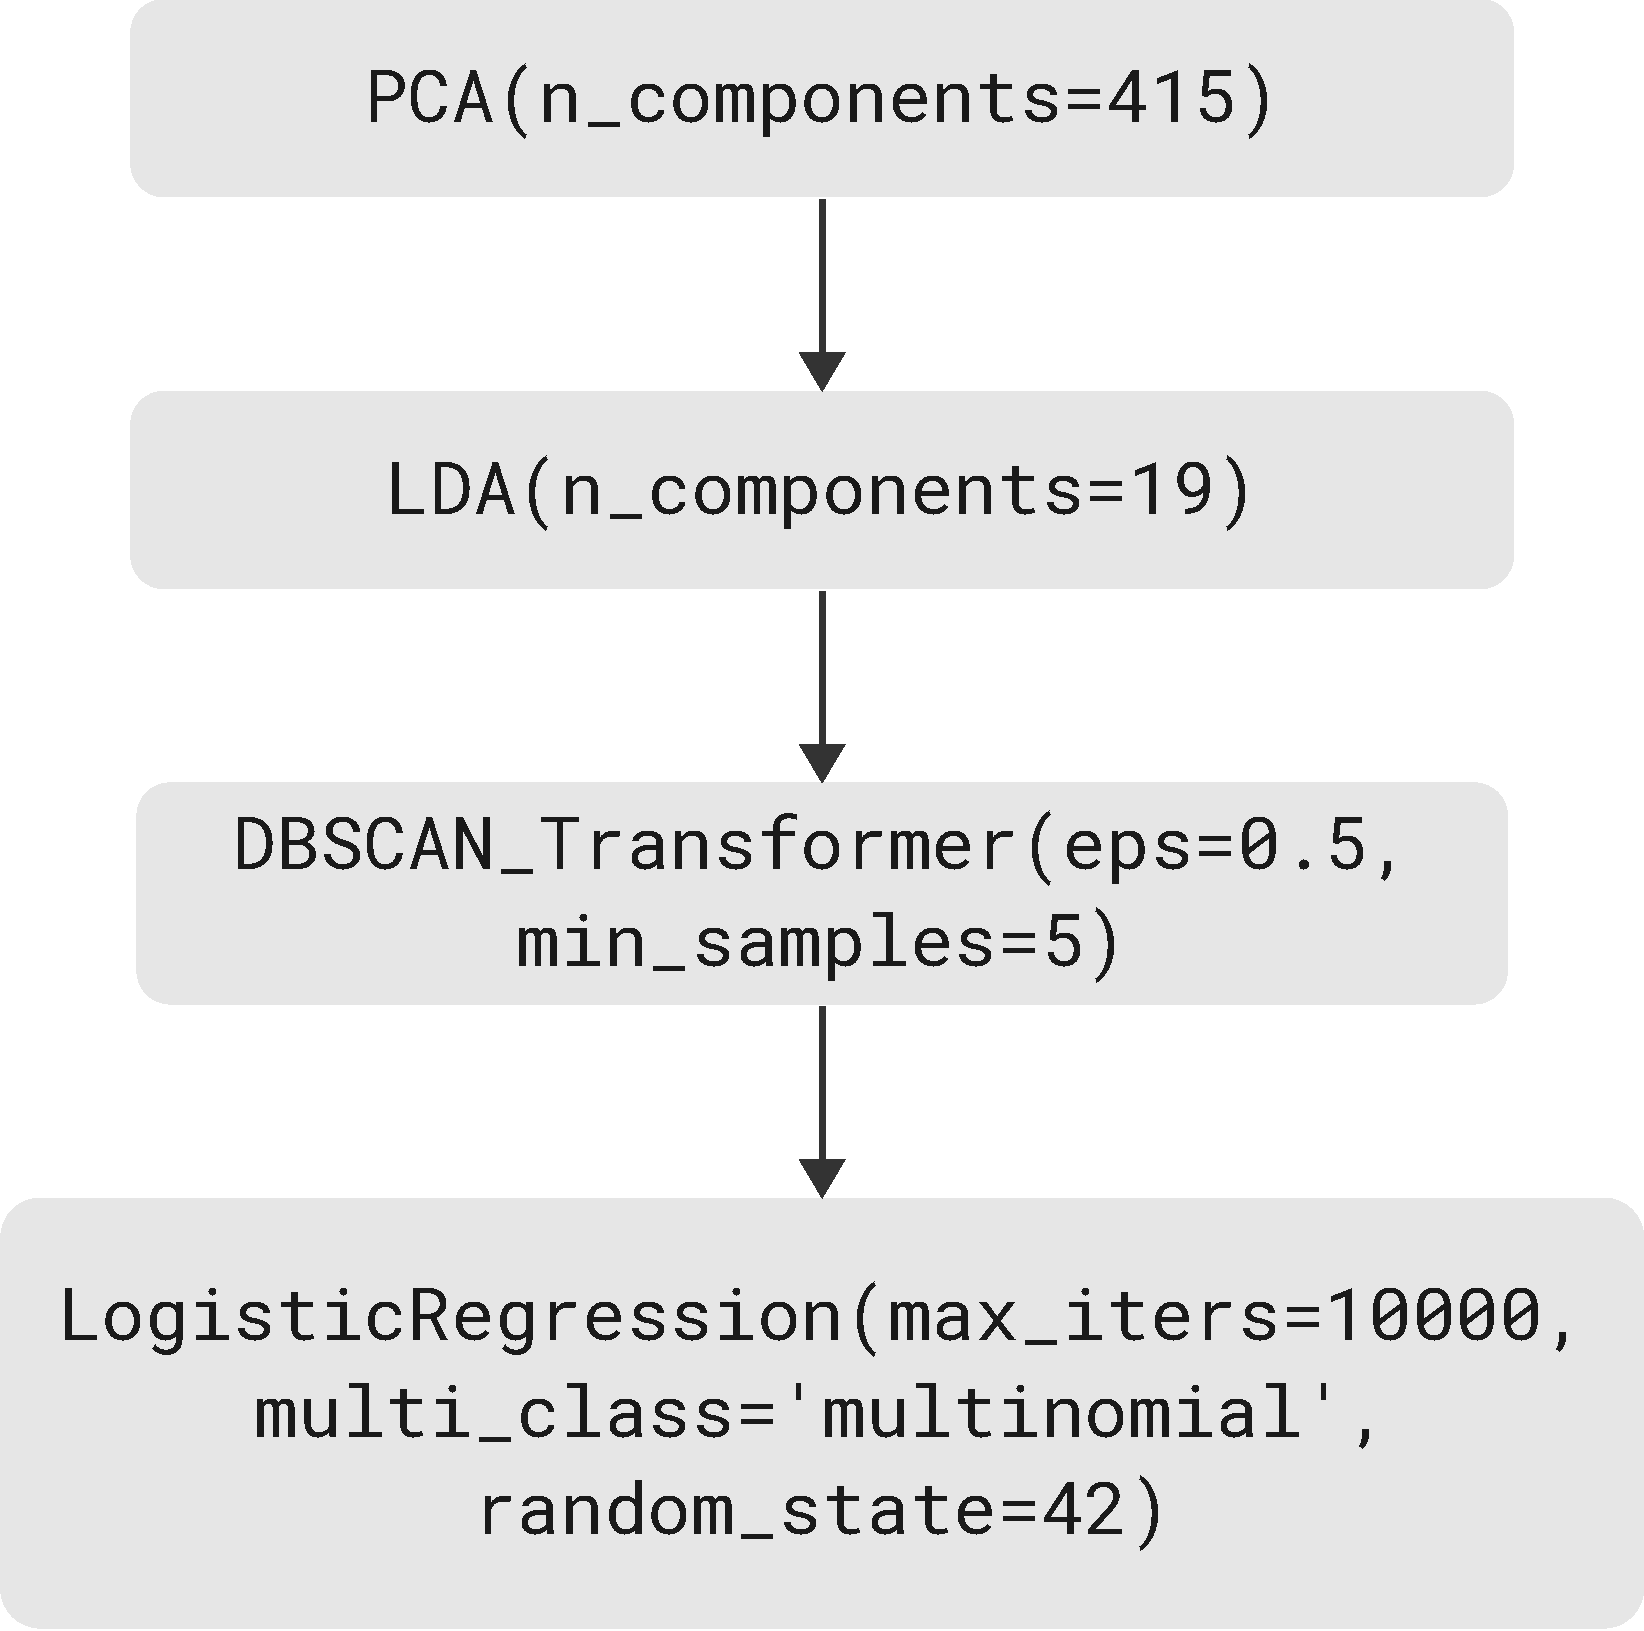
\includegraphics[width=150px]{pipeline.pdf}
    \caption{Diagramatic Representation of model pipeline}
    \label{fig:my_label}
\end{figure}


\section{Ensembling Methods}
Ensemble methods combine the predictions of multiple models while improving the overall prediction accuracy. Bootstrap Aggregation (bagging) \cite{bagging} is a common technique used to reduce variance and overfitting in machine learning algorithms. Other ensemble techniques include boosting \cite{boost} and stacking \cite{stack}. These techniques have been applied in various domains, such as sentiment analysis, credit scoring, and recommendation systems.


During the training process, the algorithm demonstrated high accuracy ranging between 99 per cent and 100 per cent on the training data. In comparison, the validation accuracy remained between 76 per cent  and 79 per cent. This discrepancy implied that the classifier might have been overfitting on the training data, indicating a high variance model. To address this, we attempted to employ the variance-reducing technique of bagging. Surprisingly, the utilization of ensembling techniques did not improve the results. Better outcomes were obtained without the use of bagging.

\section{Conclusion}

The best-performing model was achieved by combining supervised and unsupervised learning techniques. Dimensionality reduction was performed using PCA with the top 415 components, followed by LDA with the top 19 components. Clustering was done using DBSCAN with \texttt{minpts=5} and \texttt{eps=0.5}, and the output labels were added as another feature to the dataset. Finally, a multinomial logistic regression classifier was fit on the data with a maximum of 10,000 iterations. The hyperparameters for each technique were tuned extensively to obtain the best results.

 
% \bibliographystyle{plain}
\begin{thebibliography}{00}

\bibitem{image} Deewakar Chakraborty, "Image Compression using Principal Component Analysis (PCA)", \url{https://www.section.io/engineering-education/image-compression-using-pca/}

\bibitem{face} Kyungnam Kim, "Face Recognition using Principle Component Analysis", \url{http://staff.ustc.edu.cn/~zwp/teach/MVA/pcaface.pdf}

\bibitem{bio} Shuangge Ma, Ying Dai, "Principal component analysis based methods in bioinformatics studies."


\bibitem{lof} Scikit-learn, "Outlier detection with Local Outlier Factor (LOF)",  
\url{https://scikit-learn.org/stable/auto_examples/neighbors/plot_lof_outlier_detection.html}

\bibitem{iso_for} Scikit-learn, "Novelty and Outlier Detection", 
\url{https://scikit-learn.org/stable/modules/outlier_detection.html#isolation-forest}

\bibitem{fraud} Diwakar Tripathi, Yograj Sharma, Tushar Lone, Shubhra Dwivedi "Credit Card Fraud Detection using Local Outlier Factor", International Journal of Pure and Applied Mathematics Volume 118 No. 7 2018, 229-234

\bibitem{seg} Qixiang Ye, Wen Gao, Wei Zeng, "Color Image Segmentation using Density-Based Clustering."

\bibitem{dbscan} Scikit-learn, "Clustering",  \url{https://scikit-learn.org/stable/modules/clustering.html#dbscan}

\bibitem{rf} Scikit-learn, "Ensemble methods",  \url{https://scikit-learn.org/stable/modules/ensemble.html#random-forests}

\bibitem{mlp} Scikit-learn, "Neural network models (supervised)":
\url{https://scikit-learn.org/stable/modules/neural_networks_supervised.html#multi-layer-perceptron}

\bibitem{bagging} Raphael John Lamarre Townshend, "Ensembling Methods", 
\url{http://web.archive.org/web/20190214124825/https://cs229.stanford.edu/notes/cs229-notes-ensemble.pdf}

\bibitem{boost} IBM, "What is boosting?", \url{https://www.ibm.com/in-en/topics/boosting}
\bibitem{stack} Graham Harrison, "A Deep Dive into Stacking Ensemble Machine Learning" \url{https://towardsdatascience.com/a-deep-dive-into-stacking-ensemble-machine-learning-part-i-10476b2ade3}


\end{thebibliography}

\end{document}
